\subsection{Blockschaltbild}
\label{sec:Blockschaltbild}

\begin{figure}[H]
	\centering
	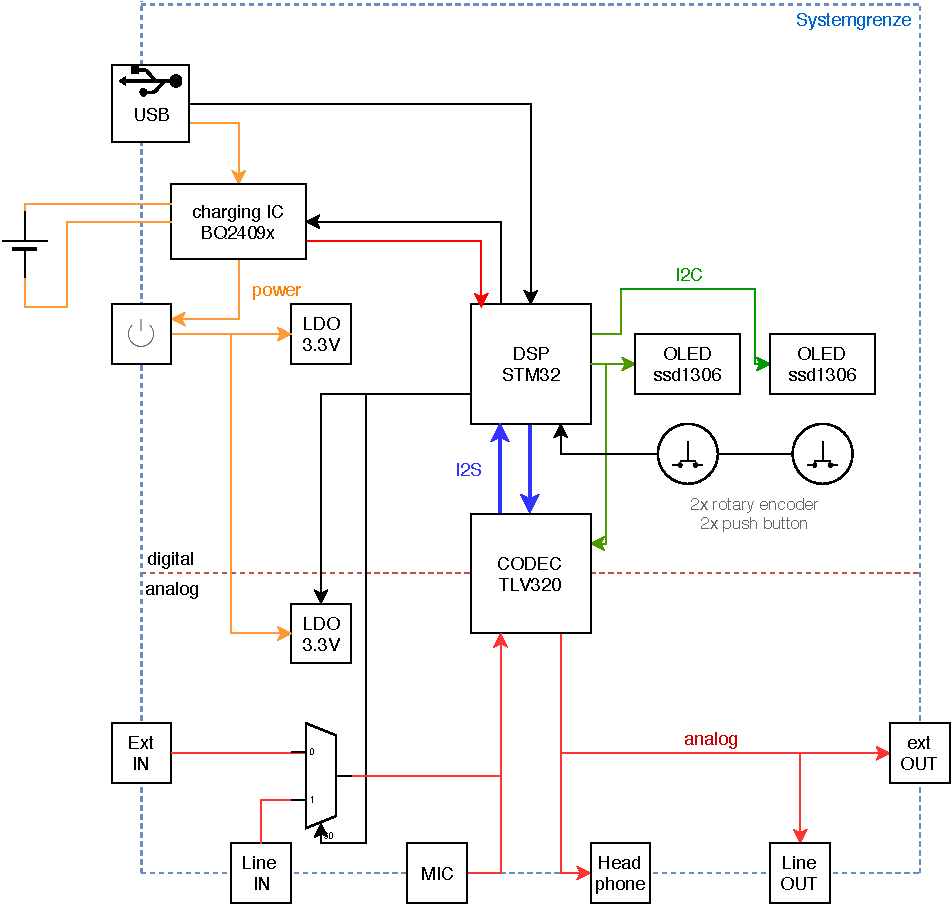
\includegraphics[width=1.0\linewidth]{block_diagramm}
	\caption{Blockschaltbild des DSP Boards}
	\label{pic:Blockdiagramm}
\end{figure}

Die Abbildung \ref{pic:Blockdiagramm} oben zeigt das Blockschaltbild mit den Komponenten um den DSP. Die Schaltung beinhaltet einen STM32 Microcontroller, dessen Beschaltung im Kapitel \ref{sec:Schema_DSP} dokumentiert ist. 
Als weitere Kernkomponente zählt der TLV320 Audio Codec, dessen Schema im Kapitel \ref{sec:Schema_Codec} beschrieben ist.

Zum Speisungsteil (orange) gehört ein Akkulade-IC (bq2409x), dessen Schaltung im Abschnitt \ref{sec:Schema_Speisung} beschrieben ist. Der Li-Ion/Li-Po Akkumulator ist auf dem Blockschaltbild ausserhalb des Systems gezeichnet und wurde im Rahmen dieses Projektes nicht evaluiert. Der bq2409x wurde gemäss Abschnitt \ref{sec:Valid_Batterie} mit einem Akkumulator getestet.




